\documentclass[runningheads,a4paper]{llncs}

\usepackage{amssymb}
\usepackage[utf8]{inputenc}
\usepackage{subfig}
\setcounter{tocdepth}{3}
\usepackage{graphicx}

\usepackage{url}
\usepackage{lingmacros}
\newcommand{\keywords}[1]{\par\addvspace\baselineskip
\noindent\keywordname\enspace\ignorespaces#1}

\begin{document}

%passwords to the submission: ID 467 klasse
\mainmatter  % start of an individual contribution

% first the title is needed
\title{A Type-Theoretical Wide-Coverage Computational Grammar for Swedish}

\author{}
\institute{}


\maketitle


\begin{abstract}
The work describes a wide-coverage computational grammar for Swedish. 
It is developed using GF(Grammatical Framework), a dependently-typed 
functional language, specialized for grammar programming. We trained
and evaluated the grammar by using Talbanken, the largest treebank for 
Swedish. As a result 65 $\%$ of the Talbanken trees were translated
into the GF format in the training stage. Moreover, we obtained a language
model for Swedish which we use for disambiguation when parsing free text
with the grammar. 
\keywords{grammar-formalism, computational grammar, treebank}
\end{abstract}


\section{Introduction}

%Motivation + brief information about Swedish+resources.

%Introduction + Aim from Master thesis(Chapter 1 + 1.1).

%Outline of the paper. 

\textbf{Ramona: Copied from the thesis, could be improved!}
GF has strong support for multilinguality and has so far been used successfully for 
controlled languages \cite{cnl}, while recent experiments have showed
that it is also possible to use the framework for parsing free language \cite{patent}.
So far there is no freely available grammar-driven parser that gives a deep
analysis for Swedish. The fact that a parser or grammar is not freely available
does not only restrict its usage but also its possibilities of being further
developed. Our goal is
to create an open-source Swedish grammar from which we derive a parser
accepting all sentences described by the given rules.
As a freely available resource, it can be continuously enhanced and
made use of in other projects.\\
\noindent To build the grammar from scratch would be not only time consuming but
would also mean that already existing systems would have to be reimplemented.
In order to not reinvent the wheel we proceed from a combination of well-tested
sources.
We start from a GF resource grammar, consisting of an abstract and a concrete syntax
file defining a set of rules for morphology and syntax.
This is what is meant by grammar in this thesis, as
opposed to grammar in the traditional linguistic sense. 
From GF, we get a well-defined system for describing language, as well as a
strong connection to and possibility of translation between the 
more than 20 other languages implemented in the framework. Further, we use
the extensive lexicon Saldo and the treebank Talbanken.

Our contribution is a wide-coverage GF lexicon, a translation of a Swedish treebank
into the GF notation and an extended Swedish grammar implementation. The grammar is based
on the multilingual abstract syntax given in the GF resource library, and now
also covers constructions specific to Swedish.
We further give an example of the advantage of using dependent types when
describing grammar and syntax, in this case for dealing with reflexive pronouns.
Grammatical Framework \cite{gfbok} is a dependently typed grammar formalism.
It is based on Martin-Löf type theory which allows
reasoning within the programming language.

Our goal is a wide-coverage grammar for Swedish which -- combined with statistical 
resources -- can be used for parsing open-domain text. The grammar implementation gives
a deep analysis, in the trade-off between coverage and depth we aim for depth
while getting coverage from statistical methods.\\

Outline ...

\section{Background}

\subsection{Swedish}

% Chapter 2.4(with emphasis on the syntactic structures)
\textbf{Too long?}
Swedish is a North-Germanic language, sharing most of its grammatical structure 
with Norwegian and Danish. It is also one of the official languages in Finland
and is spoken by approximately 9 million people.
Although Swedish syntax often is similar to English, the  morphology is richer and the
word order more intricate.
It is a verb-second language \cite[p.116]{gunlog}: the
second constituent of a declarative main clause must consist of a verb.
The normal word order is subject-verb-object, but fronting other constituents
-- topicalisation -- is very common,  especially for temporal and
locative adverbial phrases \cite[\textsection 1027]{H&H}.
Fronting the finite verb marks questions.

Swedish has two ways of forming passive verb phrases: the 
\textbf{periphrastic passive}, formed by using the modal auxiliary verb `bli' (\emph{`become'})
and the \textbf{s-passive} which is formed by adding an \emph{s} to the verb: \\
\enumsentence{Passive \hspace{45mm} Active\\
\shortexm{12}
{Tjuven & togs&  av & polisen}
{\emph{the}\emph{ thief}&  \emph{took}+\textbf{s}&  \emph{by}&\emph{the police}}
{``The thief was arrested by the police"}
{&&Polisen & tog & tjuven}
{&&\emph{the police} & \emph{took} & \emph{the thief}}
{\hspace{-9mm}``The police arrested the thief"}}
\label{gfPass:s-pass}

Special reflexive pronouns and reflexive possessive pronouns for the 3rd
exist \cite[\textsection 310 \& 319]{H&H}, distinct from the normal 3rd person forms.
\enumsentence{
\begin{tabular}{llll}
a. & Han slog \textbf{sig}.&\hspace{20mm}b. & Han såg \textbf{sitt} barn.\\
&\emph{He hit \sc self.} && \emph{He saw {\sc self's} child.}
\end{tabular}}
\enumsentence{
\begin{tabular}{llll}
a. &Han slog \textbf{honom}. &b.& Han såg \textbf{hans} barn.\\
&\emph{He hit him (another person).}&&\emph{He saw his (another person's) child.}
\end{tabular}}


\subsection{GF}
\label{sec:gf}
\textbf{Ramona: this is copied too, probably much room for improvement,
and it also has to be shortened}
%Chapter 2.1 + reference to Krasimir's work on the Penn Treebank
%(+ 2.1.3), nothing about resource library here
The main component of the project is the Grammatical Framework (GF) \cite{gfbok},
a grammar formalism based on Martin-Löf type theory \cite{martinlof}. GF is
designed for multilingual applications and represents a formalism
stronger than mildly context-free grammars. 

GF is a strongly typed functional programming language, inspired by
ML \\\cite{ml} and Haskell \cite{haskell}. It is also a logical framework,
and the built-in functionality for logic and reasoning 
is inspired by $\lambda$ Prolog \cite{prolog} and 
by Agda \cite{agda}, with which GF also shares its type checking algorithm.
The first version of the framework was implemented at Xerox Research Center
in Grenoble and is now mainly developed in Gothenburg. One of the biggest
achievements is a library covering the 
basic morphological and syntactic structures of more than
20 languages (see section \ref{sec:resources}).


A grammar written in GF can be used for both parsing and generation.
The parsing algorithm is incremental and has polynomial time and space
complexity \cite{gfMech}. 
The GF package also provides various tools for working with and using the grammars:
a compiler, an interpreter and a runtime system.
The grammars can be compiled into portable grammar format (PGF) \cite{pgf},
supported by Java, Java script, C and Haskell libraries. 
The interpreter, the GF shell, allows
the user to test grammars by commands for parsing, visualization of parse trees,
random generation, word alignment, morphological quizzes etc.
The shell can be tried out online 
together with an interactive GF editor 
\footnote{http://www.grammaticalframework.org/demos/gfse/}.
\thispagestyle{plain}
\begin{figure}[h]
\begin{verbatim} 
> parse "jag ser katten" | visualize_tree  -format=pdf -view=evince
> parse "jag ser katten" | visualize_parse -format=pdf -view=evince
\end{verbatim}
\caption{Example of how the GF shell can be used.}\label{fig:shellvp}
\label{fig:shell}
\end{figure}
Figure \ref{fig:shell} shows commands for parsing, where the results are shown as
in figure \ref{fig:gftree1}. 
GF uses Graphviz\footnote{http://www.graphviz.org/}
to visualize the trees and the given commands (fig. \ref{fig:shell}) specify that the
output format should be PDF and that these files should be opened by the program
Evince. The user can choose to see the \textit{parse tree} (fig. \ref{pic:gfStree})
or the \textit{abstract tree} (fig. \ref{pic:gfAtree}). Abstract trees are more verbose and show all
functions and types used for parsing the sentence. 
\begin{figure}[!h]
\centering
\subfloat[Swedish parse tree]
{\label{pic:gfStree}\includegraphics[width=30mm]{gfSTreec.pdf}}
\label{fig:gftree1}
\subfloat[English parse tree]
{\includegraphics[width=30mm]{gfETreec.pdf}
\label{pic:gfEtree}}
\subfloat[GF abstract tree]
{\label{pic:gfAtree}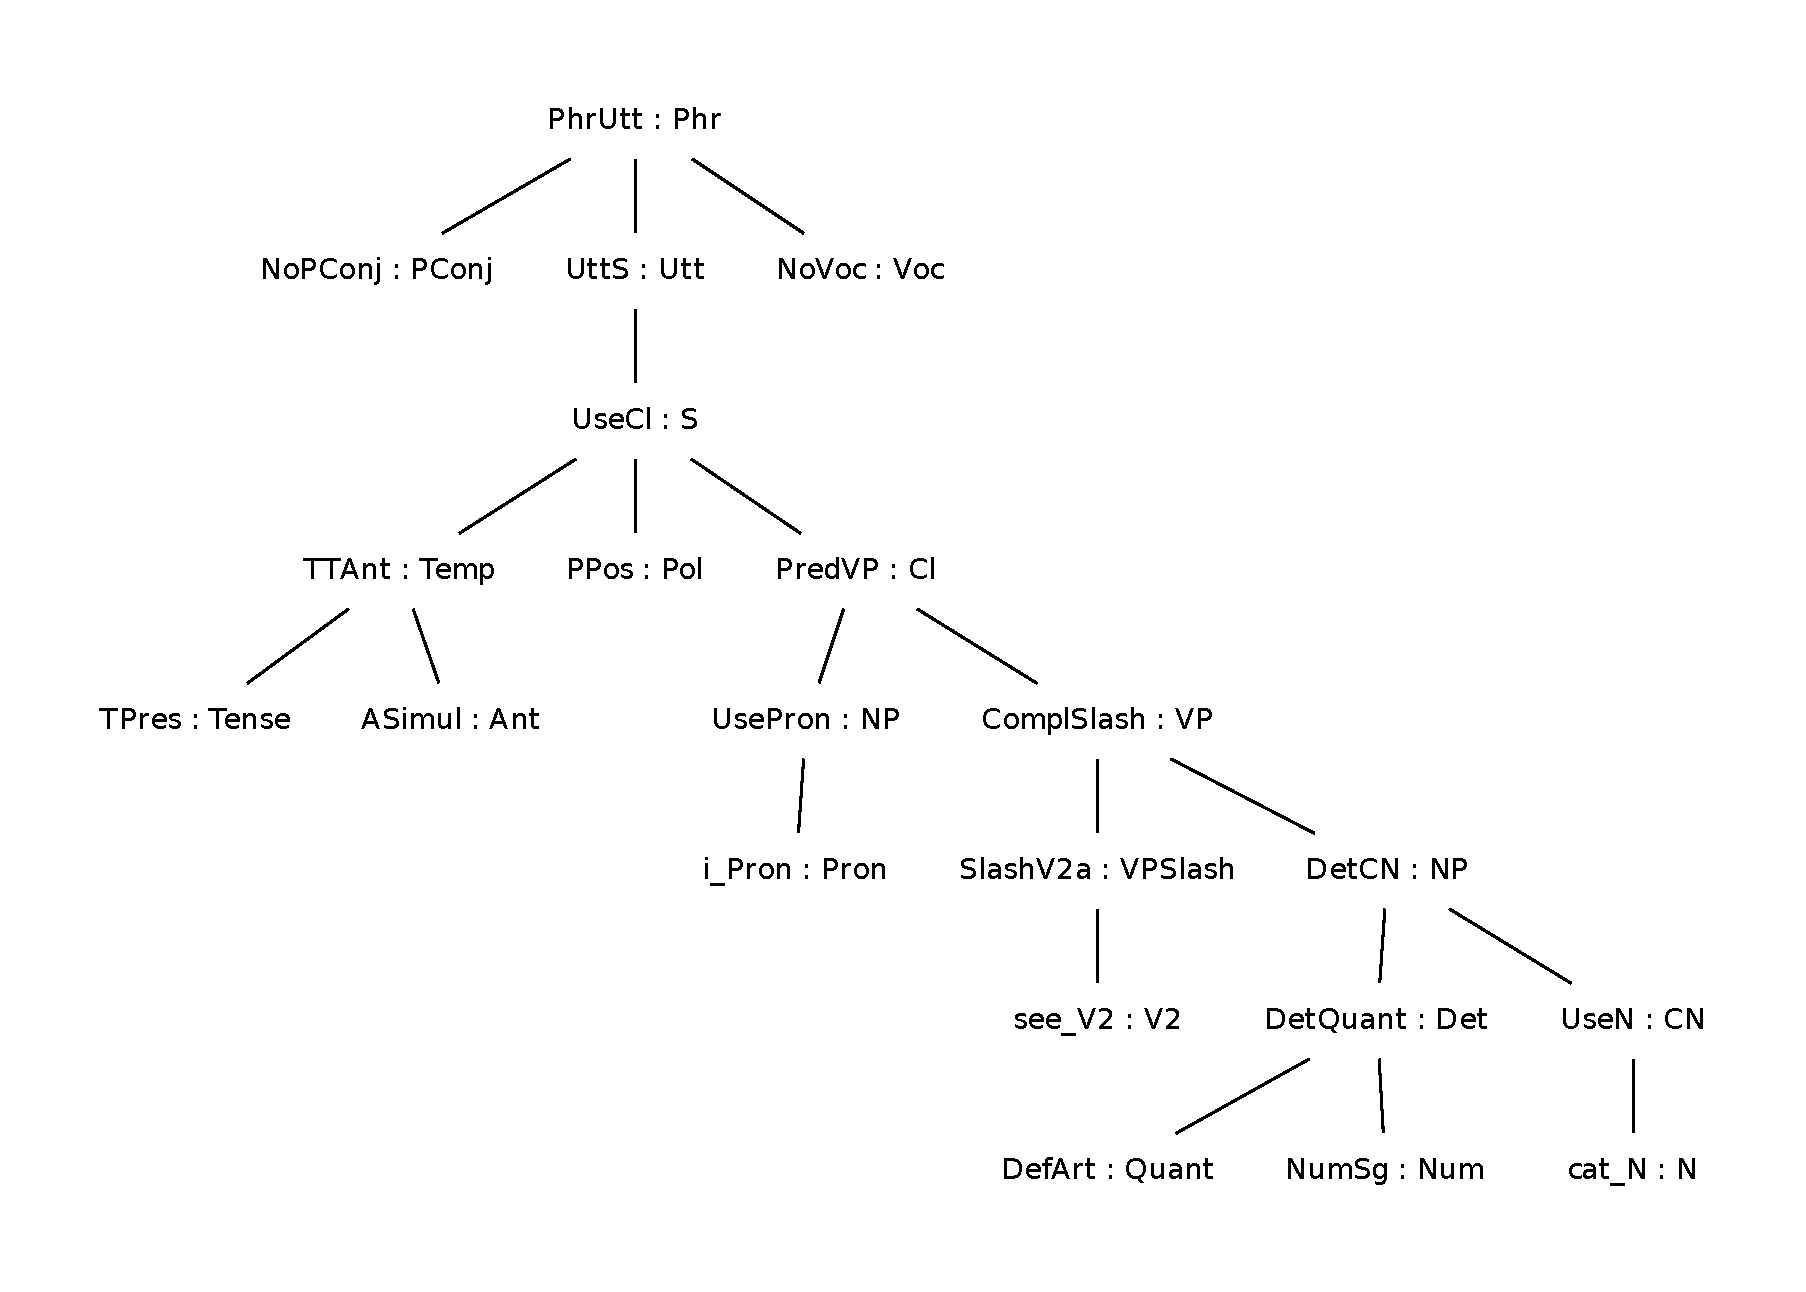
\includegraphics[width=30mm]{gfTree.pdf}}
\caption{Abstract tree and parse tree for the sentence ``Jag ser katten".}
\label{fig:gftree1}
\end{figure}
Parse trees on the other hand show only the types assigned to the words and phrases.
Information about tense, polarity etc., which are explicitly given in the abstract tree, are
not reproduced in the parse tree. Hence, parse trees do not give complete representations
but model the parse results in a transparent manner.

The scope of GF grammars has so far been controlled language, a subset of a
natural language used for a restricted domain. By
restricting the coverage, the number of ambiguities
can be limited and it can be ensured that the semantics is preserved during
translation. Inherited ambiguities as well as ambiguities arising from multilinguality will
remain, but can be controlled more easily. 

The use of controlled language thus gives the possibility of good and reliable
translation and GF has successfully been used for this in a number of projects.
WebAlt \cite{webalt} aims to develop language independent
material for mathematics problems by using GF grammars.
The formal software verification tool
KeY \cite{key} used GF for translating formal specification to
natural language.
GF has further been used for describing dialogue grammars \cite{talk}, and
the framework is one of the main component in the
European project MOLTO\footnote{http://www.molto-project.eu/}, which develop
online translation between to 15 languages.\\

As an open source-project, GF is constantly being developed and improved. New
languages are added, the compiler is being improved, ways of using it in more 
efficient and easy-going manners are added
and the possibilities to use GF in different environments
increased. There is research on how to make more use of the dependent
types, for reasoning by using ontologies \cite{ontologies2} or generating natural
language via Montague semantics \cite{montague}.




\subsection{Talbanken}

%Chapter 2.2
\label{sec:talbanken}
For testing and evaluation of the grammar and lexicon, we needed to be able to
compare them against a reliable source.
We have used Talbanken \cite{talbanken},
a freely available, manually annotated, large-scale treebank.
It is analyzed with the MAMBA annotation scheme (Teleman, 1974) and 
consists of four
parts. Two of them are transcriptions of spoken language, one a collection of
text written by high school students, and one, section P,
consists of professionally written Swedish gathered from newspapers, brochures and textbooks.
\\
\noindent Talbanken was also used to train the Swedish version of the Malt parser \cite{malt}
and was then redistributed in an updated version,
Talbanken05 \cite{talbanken05}.
It is released in Malt\footnote{http://w3.msi.vxu.se/~nivre/research/MaltXML.html} 
and Tiger\footnote{http://www.ims.uni-stuttgart.de/projekte/TIGER/TIGERSearch/doc/html/TigerXML.html}
XML-formats
where the trees have been made deeper and more detailed while still containing
the lexical MAMBA layer. 
The Malt parser was trained on section P of Talbanken, and these
more than 6000 sentences have been used our project. 
The treebank has served as an inspiration and an evaluation source throughout the
project.



 
\section{Related Work}
\textbf{Ramona: also just copied, if you want, improve it}
%Chapter 2.5 - w/o the references about lexical resources
%
%Mention the LREC paper and what it does, without any direct reference
%between the authors
There are many other parsers for Swedish,
like the well-known data-driven Malt parser \cite{malt},
which has been trained on Talbanken. 
There are also a number of grammar-based parsers, although none is freely available.
The cascaded finite state parser CassSwe \cite{casswe} and
The Swedish Constraint Grammar \cite{birn}
give syntactic analyses. 
Swedish FDG (Voultanien,2001) uses the Functional Dependency Grammar
\cite{fdg},
an extension of the Constraint Grammar
formalism, and produces a dependency structure focusing on finding the nominal
arguments.

The LinGO Grammar Matrix \cite{matrix}, is a starter-kit for building Head-Driven Phrase
Structure Grammars \cite{hpsg} (HPSG) providing compatibility with tools for
parsing, evaluation, semantic representations etc.
Translation is supported by using Minimal Recursion
Semantics \cite{mrs} as an interlingua. \\
There is a collection of grammars implemented in this framework, giving broad-coverage
descriptions of
English, Japanese and German.
The Scandinavian Grammar Matrix \cite{scandmatrix} covers common parts of
Scandinavian, while Norsource \cite{norsource} describes Norwegian. A Swedish version
was based upon this (SweCore, Ahrenberg) covering the morphology and some
differences between Swedish and Norwegian. Further, there is the BiTSE 
grammar \cite{stymne}, also implemented using the Lingo Matrix,
which focuses on describing and translating verb frames.

The Swedish version of the Core Language Engine (CLE) \cite{gamback}
gives a full syntactic analysis as well as semantics represented in `Quasi logical form'. A
translation to English  was implemented and the work was further developed in the spoken
language translator \cite{spoken}. Unfortunately, it is no longer available. The coverage of the Swedish

In the TAG formalism \cite{tag}, there are projects on getting open source, wide-coverage grammars
for English and Korean, but, to our knowledge, not for Swedish.  

The ParGram \cite{pargram} project aims at making wide coverage grammars using
the Lexical Functional Grammar approach \cite{lfg}.
The grammars are implemented in parallel in order to coordinate the analyses of
different languages and there are now grammars for English, German, Japanese and Norwegian. 



\section{Grammar}

%Discussion about the two dimensions of a grammar - lexicon and syntax 
There are to aspects of on a computational grammar clearly distinctive (?)  in
our work- the work on the lexicon and the work regarding syntax.
For this article, we will focus on the syntactical dimension, the description
and formalization of grammar rules and the usage of Talbanken.

\subsection{Resource grammar}

%Chapter 2.1.2
The GF package provides an useful resource library \cite{gf-resource}, covering the
fundamental morphology and syntax of more than 20 languages.
There is also a small test lexicon included, containing a few hundred common
words.
Since the languages all share the same abstract syntax translation between any given
pair is possible, which is valuable
when implementing multilingual applications.

The resource grammars describe how to construct phrases and sentences and how to
decline words. The grammars cover the morphology,
word order, agreement, tense, basic conjunction etc.
Due to the syntactic similarities of the Scandinavian languages, much of the implementation
is shared with Norwegian and Danish. The modules that concern the lexical
aspects are separate, while 85 \% of the syntax description is shared.
There are about 80 functions, which describe the rules for building phrases and clauses.
\begin{verbatim}
PredVP       : NP -> VP -> Cl ; -- Predication
ComplVPSlash : VPSlash  -> VP ; -- Complementation
\end{verbatim}
The analysis preformed by GF is driven by the parts of speech, which are combined into
parts of sentences.
In addition to the core resource grammars, which is shared with the other languages implemented in the
library, there is also an extra module, simple called the \verb|Extra| module, where
 language specific constructions may bee added
The functions given here do not have to be translatable
to all other language, but are meant to cover language specific constructions.


\subsection{Lexicon}

%Everything about Saldo, Lexin, etc, compressed.
%
%We use the resources from the other paper, so to say :)
\textbf{Some more here}
Our main lexical resource is SALDO \cite{}. We use the tools
described in \cite{} to extract a large-scale lexicon and annotate
this with valencies from Lexin. This gives us a dictionary with more than 
100 000 entries, covering all but 500 words from Talbanken ignoring names,
numbers and compounds.

\subsection{New Features}

%Section 4.2
%
%Selection of additions to the grammar 
%
%- reflexive possesive pronouns
%
%- s-passive
%
%- impersonal constructions
%
%- miscellaneous 
It has earlier been hard to identify missing constructions of the Swedish
implementation since there was no large resource available to evaluate it on.

Our evaluations are based on Talbanken and when first conducting tests
 we found much room for improvement. The items listed below are examples
 of constructions implemented during this work.

\textbf{shorten these sections}
\subsubsection{The s-passive}
Passive voice is often used in Swedish, especially the
\textit{s-passive} as described in ....
Some studies suggest that the s-passive is used in more than 80 \% of the times
\cite{laanemets}.
It is however not as common in the other Scandinavian languages, 
where not all words have passive forms for all tenses. The resource grammar for
Scandinavian therefore implemented the function for passive,
\verb-PassV2-, by using auxiliary verb.
The function allows two-place verbs to be used in passive by using \emph{bli} (\emph{become}), and thereby
turned into complete verb phrases; they no longer need an object.
During this project, the s-passive was added although the
periphrastic passive is still allowed.
The grammar further allows not only transitive verbs, but all verb phrases that
misses an object, to form passives.
A ditransitive verb -- `give' (\ref{sent:give2pass}) -- hence gives rise to two
passives, (\ref{ex:passV32}) and (\ref{ex:passV33}).
\enumsentence{\textbf{Active use of two-place verb}\\\shortex{4}
{Vi & erbjöd& henne& jobbet }
{\emph{we} & \emph{offered}& \emph{her}&\emph{the job}}
{``We offered her the job"}}
\label{sent:give2pass}
\enumsentence{\textbf{First place in two-place verbs}\\\shortex{3}
{Hon & erbjöds & jobbet}
{\emph{she} &\emph{ offered+\textbf{s}}&\emph{ the job}}
{``She was offered the job"}}
\label{ex:passV33}
\enumsentence{\textbf{Second place in two-place verbs}\\\shortex{3}
{Jobbet & erbjöds & henne }
{\emph{the job} & \emph{offered+\textbf{s}}&\emph{ her}}
{``The job was offered to her"}}
\label{ex:passV32}


\subsubsection{Impersonal constructions}
\label{sec:Formal}
Formal subjects \cite[\textsection 19]{SAG} are often used in Swedish.
\enumsentence{\shortex{6}
{Det & sitter & en & fågel & på & taket}
{\emph{it }& \emph{sits }& \emph{a} & \emph{bird} &\emph{ on} & \emph{the roof}}
{``There is a bird sitting on the roof''}}
\emph{`Det'} has the position of the subject, and the real subject, 
\emph{`en fågel'} the one of an object.

Both the verb and the noun phrase have some restrictions: the determiner of the
noun phrase must be of such type that it requires both the noun and its modifiers
to appear in indefinite form. The verb phrase must consists of a intransitive verb
or be in passive form.
A very common example of impersonal constructions is sentences with the verbs \emph{finnas},
(\emph{exist})
\emph{saknas} (\emph{miss}) and \emph{fattas}(\emph{lack}).
\enumsentence{\begin{tabular}[t]{@{}*{18}{l@{\ }}}
a. &Det & finns & kaffe &&&
b. &Det & saknas&  kaffe &&&
c. &Det & fattas & kaffe \\
&\emph{it }& \emph{exist }& \emph{coffee} && &
 &\emph{it }& \emph{misses} & \emph{coffee} && &
 &\emph{it} & \emph{lacks} & \emph{coffee}\\
\end{tabular}\\
{~~''There is coffee"~~~~ ''There is no coffee"~~~~ ''There is no coffee"}}

\subsubsection{Formalizing the rules for reflexive pronouns by using dependent types}
\label{sec:reflexives}
An important area in a Swedish grammar is the treatment of the reflexive pronouns and
the reflexive possessive pronouns.
The reflexives require an antecedent with which they agree in
number and person.
The third person reflexives requires a third person antecedent and
reflexive pronouns can not be used in subject noun phrases of finite sentences,
as shown by the ungrammatical examples in 
sentence (\ref{ex:ReflGenB}) and (\ref{ex:ReflSubj}).
Furthermore, the antecedent must be within the same finite sentence as the reflexive
pronoun, see (\ref{sent:sesig}).

Still our grammar should accept the sentences (\ref{ex:ReflGen}),
(\ref{sent:rakasig}) and (\ref{ex:ReflAdv}) :

\eenumsentence{
\item
{Sina vantar hade han glömt på tåget.\\
{\sc self's} gloves, he had forgotten on the train.}
\label{ex:ReflGen}
\item
{*Sina vantar var kvar på tåget.\\
{~~ \sc self's} gloves was left on the train.}
\label{ex:ReflGenB}}
\eenumsentence{
\item{
Jag vill att han rakar sig.\\
I want him to shave {\sc self}.}
\label{sent:rakasig}
\item
{*Han vill att jag ser på sig.\\
~~He wants me to look at {\sc self}.}\label{sent:sesig}
}
\eenumsentence{
\item{
Han är längre än sin kompis.\\
He is taller than {\sc self's} friend.
}\label{ex:ReflAP} \label{ex:ReflAdv}
\item{*Han och sin kompis läser en bok.\\
He and {\sc self's} friend are reading a book. }
\label{ex:ReflSubj}
}

In the standard GF analysis, which is preformed bottom-up starting from the
POS-tags, information about semantic roles are given by the functions, not by the
categories. That is, we know that the first argument of the function
\verb-PredVP- acts as the subject, but the noun phrase itself does not carry
information about its semantic role.
As noun phrases containing reflexive pronouns may be used as ordinary
noun phrases, apart from the restrictions stated above,
we do not want them to differentiate
from other \verb-NP- on the type level since we would then need to duplicate
our code, due to the rich type system in GF. Still, we need the type system to
help preventing noun phrases containing reflexive pronouns to be used as subject.
This does not only concern noun phrases, but also adverbial and adjectival phrases 
(\ref{ex:adjTyp} a,b).
\eenumsentence{
\item{
taket på sitt hus\\
\emph{the roof of {\sc self's} house}}
\item{
längre än sin kompis\\
{\emph{taller than {\sc self's} friend}}}}
\label{ex:adjTyp}

The solution chosen introduce the use of dependent types.
We make a difference between subjects and objects, but not
by giving them entirely different types, but by 
letting the type \verb-NP- \textit{depend} on an argument, which may either be \verb-Subject- or
\verb-Object-.
\begin{verbatim}
PredVP       : NP Subject -> VP        -> Cl ; -- predication
ComplVPSlash : VPSlash    -> NP Object -> VP ; -- complementation

-- adverbial phrases 
PrepNP      : (a : NPType) -> Prep -> NPTyped a -> AdvTyped a ; 
\end{verbatim}

We hence combine the-part-of-speech driven analyse normally preformed by
GF with a part-of-sentence analysis, where the dependent types gives the 
information we were missing.

The dependent types in GF have been used for logical reasoning before but this 
is the first example of using it in a grammar describing pure syntax of
a natural language. Other languages having similar relations between 
noun phrases and antecedent could be extended to use the type system in similar
ways.

\subsubsection{Overgenerating}
Another aspect of the grammar implementation was the avoidance of overgeneration. As
the Swedish resource grammar had not been used for larger projects, many examples of
overgeneration were present that did not cause problems when working with small
lexicons and controlled languages, but that caused explosions of ambiguities when 
tested on Talbanken. For the function \verb-GenNP-, used for genitive, we managed
to decrease the number of parse trees for some sentences to 10 \%.
% Could also be here:
%Experiments were also conducted on how we can use Talbanken for assigning correct
%types to words which we couldnot import directly from SALDO, due to annotational
%differeneces.


\section{A GF Treebank for Swedish}
\label{sec:mapping}

%Chapter 5 - short introduction about Talbanken tags + difference in
%the tags + 5.2(the translation process - first part) + example of
%2 trees  
Why we do this...... when is meta used
Talbanken05 uses three kinds of tags: categories, edge labels and POS-tags. 
While the POS-tags are reserved for words, the categories give grammatical information,
such as \verb|S|, \verb|NP| and \verb|VP|.
The edge labels give the
part of sentence: \verb|SS| for subject, 
\verb|OO| for object etc. Nearly 400 different tags are used, of which more than
300 different are POS-tags. The high number is due to the level of detail,  there are for
example almost 50 tags for nouns, excluding proper names. The tags
show definiteness, case and whether the word is a compound. Some words also have
their own tags.\\

\begin{tabular}{lll}
\textbf{Tag} & \textbf{Example} & \textbf{Explanation} \\
\hline
\textbf{SV} & \emph{ska} (`shall') & The verb \emph{shall}\\
\textbf{NNDDHSGG} & \emph{familjemedlemmarnas} & Noun, definite, compound (person),\\
&(`the family members' ') &genitive \\
\textbf{XX} & & Unclassifiable part-of-speech\\
\end{tabular}\\

The mapping could in some cases be performed tag-by-tag, but annotational
differences complicated the translation.
One example is valency information, which is given implicitly by the complements
of a word in Talbanken. If a verb is followed by an object, \verb-OO-, which contains an
\verb-S-, we can conclude that this is a sentence-complement verb.
In GF, the valency information is given for each entry in the lexicon.
A sentence-complement verb has the type \verb-VS- and from this we know 
that the function \verb-ComplVS- should be used to combine the verb and with a 
sentence.
Another annotational difference that turned out to be problematic for the
translation can be illustrated by analysis of the generic pronoun \emph{`man'}.
In Talbanken, \emph{`man'} is simply a personal pronoun, 
in GF it is represented by using the function \verb|GenericCl| which turns a
\verb-VP- into a clause and has no subject visible in the abstract tree. 

When translating a sentence like this, it is thus not possible to simply glue the
subject to the verb with \verb|PredVP|. For each similar GF construction, an extra rule
would be needed to get full coverage. 

The tags \textbf{XX} and \textbf{NAC} (\verb-Not a constituent-) are often used since Talbanken makes a
difference between subject
and object noun phrases.
The analysis of elliptical expression in (\ref{sent:krav})
\enumsentence{För stora krav.\\
``Too high demands."}\label{sent:krav}
contains both these tags, since it is not obvious
whether the noun phrase is used as subject or an object.
These tags occur quite frequently in the treebank and are always translated
to metas, which lowers our result. \\

The evaluation measures the numbers of \textit{metas} in each translated tree.
If the finite verb is untranslatable, we get metas for the verb itself and for the
tense.
For all of Talbanken, we get a number of 65 \%, and if we limit our input to
uncomplicated sentences with no more than 10 words where all words are known to
our lexicon, we can reach 85 \%. When translating the whole treebank, 78 sentences
could not be mapped at all and resulted in \textit{metas} only.

\section{Chunk Parsing}

%New section - insights about latest work
The grammar, which is hand written, cannot be expected to cover all
possible expressions of the language.
Hence, we combine it with statistical means to get good coverage. Our approach
makes use of the rich annotation in Talbanken -- we perform chunk parsing
relying on some of the tags given in the treebank. 
Unknown words and grammatical constructions, idioms or ellipses cannot be
handled from within the grammar.
Therefore, whenever a sentence is not recognized by the grammar, it is 
parsed chunk by chunk.
Noun phrases, adverbial phrases and ? are considered. At the first stage,
we try to parse the basic sentence structure, and therefore allow the parser
to parse complicated chunks as dummy words. This way, we don't loose the 
high-level sentence analysis given by GF.
When this is done, we try to separately parse the chunks,
until as much of the sentence as possible is covered. 

This way we get good coverage -- from ca 10 \% of Talbanken -- to ??

\section{Language Model-Based Disambiguation}

 Maybe move this to future work, we have it but not really sure
 if it is actually used atm.

%New section - fill in with the basic principle + new results(when available)
The translation of Talbanken to GF gives us a GF treebank consisting of more than
6000 sentences. The translation process is explained in section
\ref{sec:mapping} and even though most trees are incomplete, that is contain
meta-variables, they still give valuable 
information about which words from our lexicon that have been used
and which functions that are needed to parse the sentence.
GF has built-in support for probabilities, and when feeding the output
from the mapping to our grammar, we get a model of the language. We believe
this data can be trusted as it is extracted from manually annotated 
real-world sentences.

This model is used for disambiguation: the parse trees for each sentence
are ranked by the sum of the probability of each function used.

\section{Evaluation}

Section 5.3 + the evaluation part from 6.1 

Latest results from chunk parsing and disambiguation

\section{Future Work}
%From 6.2 subtract the things that are already done, maybe more future
%work related to the results for chunk parsing and disambiguation. 

abbrivations, idioms, learning adVs.
\textbf{too much about grammar details? there should be other things here as well}
At the end of the current project, we are left with 
many interesting future directions.
 
\subsubsection{Grammar}
The grammar should cover the most prominent Swedish features.
Even as some work must be left for the robustness, there are specific constructs
that are desirable and interesting to implement. A few examples are listed here:\\

\begin{itemize}
\item
\textit{Pronominal object shift} is common in Swedish and obligatory in Danish and Norwegian.
\enumsentence{\begin{tabular}[t]{@{}*{11}{l@{\ }}}
a. & Jag & ser&  honom& \textbf{inte}&~~ & b.&Jag &ser &\textbf{inte} &honom\\
   & \emph{I} & \emph{see}&\emph{him}&\emph{not}&&& \emph{I} &\emph{see}&\emph{not}&\emph{him}\\
\end{tabular}}
Personal pronouns are allowed to precede negation and some other sentence adverbials % --\textit{satsadverbial} --
in main clauses without auxiliary verbs.

\enumsentence{\begin{tabular}[t]{@{}*{12}{l@{\ }}}
a. & *Vi & har&  honom&  inte&sett&~~ & b.& * Jag &ser &huset &inte\\
   & \emph{~we} & \emph{have}&  \emph{him}&  \emph{not} &  \emph{seen} && b.& \emph{~I}&\emph{see} &\emph{the house} &\emph{not}\\
\end{tabular}}

Although object shifts are frequently used, they are hardly found in
Talbanken's part P, which has been the inspiration for this project.
Therefore, this implementation has so far not been prioritized.\\

\item
\textit{Bare indefinites} are at this point always parsed as mass nouns
    \enumsentence{\shortexnt{3}
{Jag & dricker& vatten}
{\emph{I}&\emph{drink}&\emph{water}}
}\label{sent:water}
although this clearly is a unsatisfying analysis for bare indefinites as in (\ref{sent:hund})
\enumsentence{\shortex{4}
{Vi & ska& köpa & hund}
{\emph{we} &\emph{will}& \emph{buy} & \emph{dog} }
{``We are going to buy a dog"}}\label{sent:hund}
\vspace{3mm}

\item
\textit{Object and subject control verbs}
The implementation of reflexive pronouns can be improved.  
It should for example be possible to differentiate between 
object and subject control verbs.

\eenumsentence{
\item[a]\shortex{7}
{Han & ber & henne & att & städa & sitt & rum}
{\emph{he} & \emph{begs} & \emph{her} & \emph{to} & \emph{clean} & {\sc self's} & \emph{room}}
{``He asks her to clean her room"}
\item[b]\shortex{7}
{Han& lovar& henne& att& städa &sitt & rum}
{\emph{he}& \emph{promises}& \emph{her}& \emph{to}&  \emph{clean} &\sc self's&\emph{room}}
{``He promises her to clean his room"}}
\end{itemize}

\subsubsection{Lexicon}
\label{sec:futureValency}
\begin{itemize}
\item When using GF for parsing with lexicon of our size, we currently
suffer from memory usage problems. The parsing algorithm is not fully
capable of evaluating all possible parse trees, which is necessary in order
to find the best one.

\item
Many Swedish verbs can be used with different number of arguments.
Having one lexical entry for every possible usage of a verb
does not seem to be a good idea considering
the ambiguities it will lead to and the already high time usage.
The task should instead be left to the robust layer of the parser, possibly
implemented by using external resources.

\end{itemize}


\section{Conclusion}
%From 6.1 - the discussion part + something about the latest work

The project has resulted in
\begin{itemize}
\item an extended grammar covering an important part of Swedish
\item a comparison between GF and another annotation
\item a deeper testing of the Swedish resource grammar and an estimation
of how well GF can be used to describe larger parts of a language
\item a study of how dependent types can be used in the resource grammars
\end{itemize}

The grammar has been extended and enhanced, and its current status is
a specialized extension of the resource grammar.
Besides parsing, the grammar may well be used for language generation,
which works fast even when using an extensive lexicon.
Although it is not been formally verified, we believe that the majority of the
sentences generated are grammatically correct in a syntactical point of view.
Without any semantic knowledge, nonsense phrases cannot be avoided in
random generation. However, given that the abstract tree has a meaningful
interpretation,
the linearization should be correct. \\

Here we have some nice new results... (todo..)

\bibliographystyle{splncs}
\bibliography{FinBib}

\end{document}
